%!TEX program = xelatex
\documentclass[UTF8]{ctexbeamer}
\usetheme{Singapore}
\usecolortheme{seahorse}
\title{动态DP}
\author{wxt1221}
\date {2023 SWOI暑假集训}

\begin{document}
\frame{\titlepage}
\begin{frame}
	\frametitle{Table of Contents - 目录}
	\tableofcontents
\end{frame}
\section{前提知识}
	\begin{frame}
		\frametitle{前提知识}
		学好动态DP,你需要了解
		\begin{itemize}
			\item 线段树
			\item 重链剖分
			\item 广义矩阵乘法
		\end{itemize}
	\end{frame}
	\begin{frame}
		\frametitle{线段树}
		运用BIT的思想可以划分区间,将整个区间分为一半,一直这样操作,于是可以推出下面的图:
		\begin{figure}[h]
			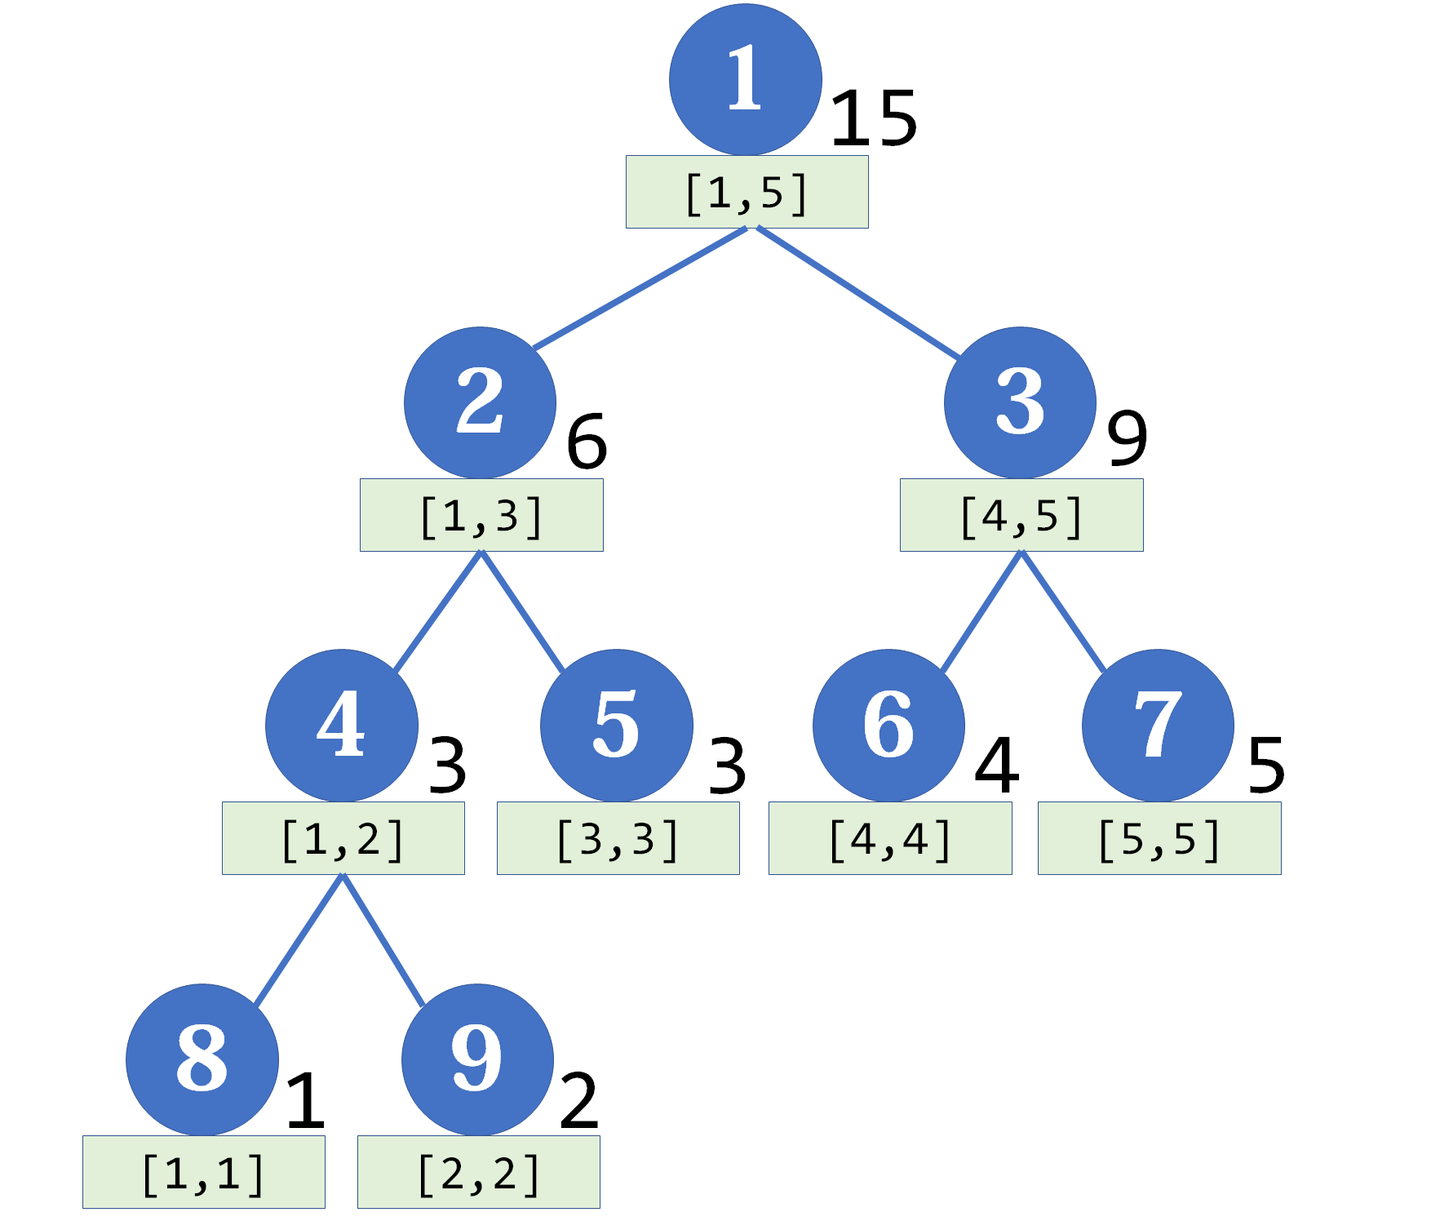
\includegraphics[width=4cm]{1.png}
		\end{figure}
		处理出每个节点的区间值即可,区间查询是 $log_n$ 级别。
		
		但是区间修改很慢,但是在这个节点的区间完全包含在需要更改的区间内,可以不用向下递归,打懒标记即可,需要使用时向下传即可。
	\end{frame}
	\begin{frame}
		\frametitle{重链剖分}
			树可以裂解为若干个线性表,但是直接处理每一条链是不优雅而且时间复杂度高,是否可以构造出一个dfs序列使得满足某些条件的节点在一起呢?
	\end{frame}
	
	\begin{frame}
		\frametitle{引入}
			\href{https://www.luogu.com.cn/problem/P3384}{\textcolor{blue}{P3384}}
			
			很明显树上任意两个节点 $a,b$ 的简单最短路径可以分解为从 a 到 $lca_{a,b}$ 和从 $b$ 到 $lca_{a,b}$ ,很明显可以考虑转换为序列上的问题,为了满足一个子树内的节点在一起,可以考虑DFS序,但是从一个节点到祖先的节点很明显不能直接放在一起,可以退而求其次,是否可以分成数量比较少的呢?
	\end{frame}
	
	\begin{frame}
		\frametitle{重儿子}
			很明显如果直接按照输入顺序进行DFS,一条路径很可能每个节点都不相邻,所以是否可以考虑按照一定的顺序进行DFS,比如按照子树大小,所以在进行DFS时,先进入子树较大的节点,此为这个节点的重儿子,连接重儿子的边称为重边,若干条(可能为 $0$)重边首尾相接构成重链。
	\end{frame}
	
	\begin{frame}
		\frametitle{时间复杂度}
			结论:从根节点到叶子结点最多经过 $log(n)$ 条重链。	
			
			\hspace*{\fill}
			
			
			\hspace*{\fill}
			
			\hspace*{\fill}
		
			证明:重链的切换的主要过程在于经过非重边,每次经过非重边子树大小必然至少除以 $2$。
	\end{frame}
	
	\begin{frame}
		\frametitle{广义矩阵乘法}
			矩阵乘法的基本形式是 $A \times B=C$ 是:$C_{i,j}=\sum_{k=1}^{n}(A_{i,k}\times B_{k,j})$
			
			其实求和以及乘法都可以被替换为其他运算。
			
			满足结合律,证明略。
	\end{frame}
\section{引入}
	\begin{frame}
		\frametitle{不考虑修改操作}
			\href{https://www.luogu.com.cn/problem/P4719}{\textcolor{blue}{P4719}}
			很明显非常模版,定义 $dp_{i,0}$ 表示不选择 $i$ ,考虑 $i$ 的子树的答案,$dp_{i,1}$ 表示选择 $ i$ ,考虑 $ i$ 的子树的答案。
			
			很明显可以推出:
			
			$dp_{i,0}=\sum \max(dp_{son,0},dp_{son,1})$
			
			$dp_{i,1}= w_i+\sum dp_{son,0}$
			
			$Ans=\max(dp_{root,0},dp_{root,1})$
	\end{frame}
\section{分析}
	\begin{frame}
		\frametitle{考虑修改操作}
		首先考虑如何让dp式更好看,又是求和又是最大值,一看就不好优化,可否把求和弄点呢,考虑树链剖分中的重儿子的思想,将 dp 转移式分成两部分如下,$bson_i$ 表示 $i$ 的重儿子:
		
		$dp_{i,0}=g_{i,0}+\max(f_{bson_i,0},f_{bson_i,1})$
		
		$dp_{i,1}= g_{i,1}+f_{bson_i,0}$
		
	
	\end{frame}
	
	\begin{frame}
		\frametitle{考虑修改操作}
			接下来我们根据这个来推出 $g$ 的定义。
		
		很明显 $g_{i,0}$ 表示不选择 $i$ 不考虑重儿子 $bson_i$ 时的答案,$g_{i,1}$ 表示选择 $i$ 时不考虑 $bson_i$ 时的答案。
		但是max操作还是在,直接放进广义矩阵里面。
		
		于是定义广义矩阵乘法为:$A \times B=C$ 是:$C_{i,j}=\max_{k=1}^{n}(A_{i,k}+ B_{k,j})$
		
		于是有:
		
		$\begin{bmatrix}g_{i,0}&g_{i,0} \\g_{i,1}& -\infty \end{bmatrix} \times \begin{bmatrix} dp_{bson_i,0} \\ dp_{bson_i,1}\end{bmatrix} = \begin{bmatrix}dp_{i,0} \\dp_{i,1} \end{bmatrix}$
		
		修改操作只用修改所经过的重链的头部的父亲的 $g_{i,1}$ 即可。
		
		因为广义矩阵乘法同样满足结合律,所以线段树维护 $g$ 即可。
		
		注意为单点修改,所以完全不用加懒标记。
	\end{frame}
\section{总结}
	\begin{frame}
		\frametitle{总结}
		动态DP可以用于一些树上DP问题需要在线更改树的形态并且随时求出dp答案的题目,对于树上问题启发很大,比如修改为特殊的点权以及边权可以将题目中一些操作统一化使用动态DP求解。
		动态DP可以用于一些树上DP问题需要在线更改树的形态并且随时求出dp答案的题目,对于树上问题启发很大,比如修改为特殊的点权以及边权可以将题目中一些操作统一化使用动态DP求解。
		
		\hspace*{\fill}
		
		动态DP的思想同样可以运用的具有区间修改的DP题,本质上是将DP转移划归为广义的矩阵乘法然后套用高级数据结构实现修改。
		
		\hspace*{\fill}
		
		同时,动态DP也具有LCT做法,本文略。
	\end{frame}
\section{推荐题目}
	\begin{frame}
		\frametitle{推荐题目}
			\begin{itemize} 
				\item \href{https://www.luogu.com.cn/problem/SP1043}{\textcolor{blue}{SP1043}}
				\item
				\href{https://www.luogu.com.cn/problem/SP1716}{\textcolor{blue}{SP1716}}
				\item \href{https://www.luogu.com.cn/problem/SP6779}{\textcolor{blue}{SP6779}}
				\item \href{https://www.luogu.com.cn/problem/P4719}{\textcolor{blue}{P4719}}
				\item \href{https://www.luogu.com.cn/problem/P5024}{\textcolor{blue}{P5024}}
				\item \href{https://www.luogu.com.cn/problem/P6021}{\textcolor{blue}{P6021}}
			\end{itemize}
	\end{frame}
\end{document}
